\chapter{Kinematics and Dynamics}


\section{Design choices }

The arm operates with a servo gear reduction ratio of
30:1, a choice validated by the design’s preliminary analysis as sufficient 
to handle the required torques while maintaining energy efficiency, critical 
for prolonged field operations.The arm features three rotational joints
(R1, R2, R3), with R1 at the base (root revolution) experiencing a torque of
T1 = 2.8 Nm, and R2 bearing a torque of T2 = .8 Nm due to the cumulative
forces from the arm’s extension. 





To calculate the torque, at first we calculate the force at joints –fully 
stretched yield forces as follows, F2 = .5 Kg(mass of the stepper motor+ mass of
gearbox ) × 9.8 = 4.5 N and F3 = .3 kg (mass of stepper motor) × 9.8
= 2.98 N), resulting in gravitational force of 4.5 N and 2.98 N at R2 and
R3, respectively. And from this force value we can estimate the torque value
required for the motor to rotate. The arm’s weight distribution is optimized
for field mobility: the total weight at joint R2 is 0.5 kg (comprising the 0.3
kg NEMA 17 motor and 0.16 kg of additional components), while R3 weighs
0.3 kg, and the finger tip at the end effector has a maximum weight of 15 g
to ensure minimal load at the arm’s extremity. Lightweight materials such as
wood or aluminum should be chosen for the links, balancing durability with
the need to reduce energy consumption, as heavier materials would strain the
motors and battery life in uneven asparagus fields.


Each joint is powered by NEMA 17 motors, 
selected for their compact size and robust performance, delivering a rated torque 
of .4 Nm with gear reduction , the value stand for 12 Nm, which exceeds the 
calculated maximum torque of 3.36 Nm in the arm’s fully stretched position, even 
after applying a 30% safety margin to account for the payload, finger tip, and 
link weights in worst case scenario. This is 7.26 times more than calculated max
torque required for this application. 








\section{CAD model and simulation}


The robotic arm model, crafted in Autodesk Inventor, serves as a foundational 
design for autonomous asparagus harvesting, emphasizing precision and 
efficiency in agricultural field conditions. The model showcases a three-joint 
configuration, with a base joint (R1) featuring a robust motor assembly, 
depicted as a red and black circular component, providing the necessary torque 
for stable root revolution. The first link extends from the base to the elbow 
joint (R2), measuring approximately 0.25 m, and is supported by a blue 
structural frame to handle the mechanical stresses during operation. 

\begin{figure}
    \centering
    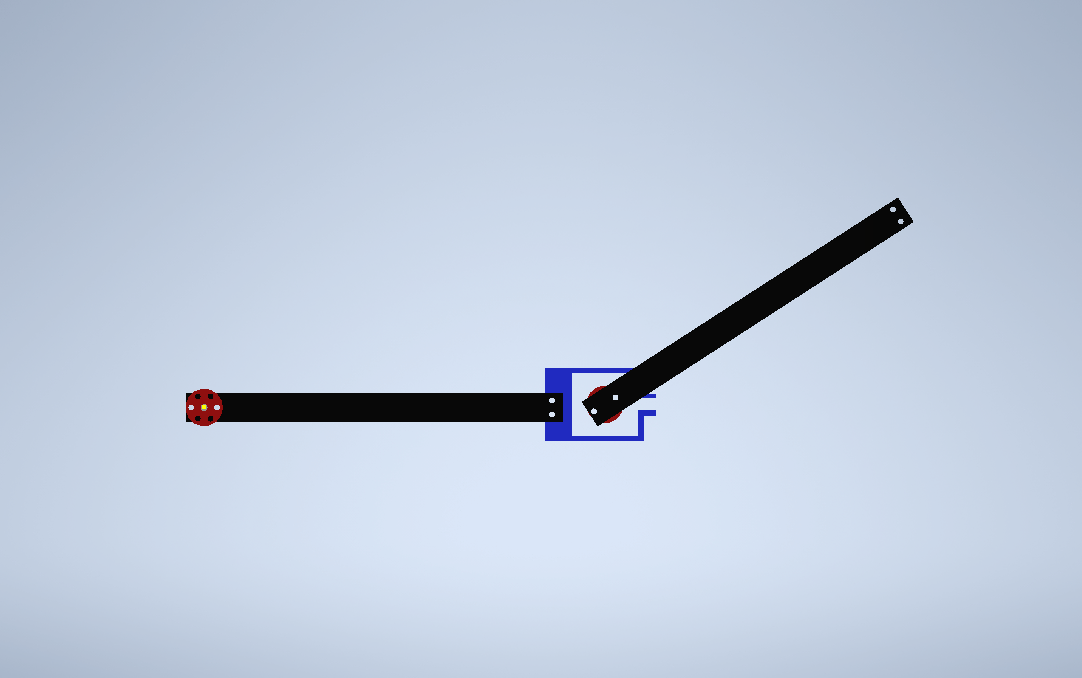
\includegraphics[width=0.75\linewidth]{inventor/inventor.png}
    \caption{robot arm design in inventor}
    \label{fig:enter-label}
\end{figure}




The second 
link, spanning 0.2 m from the elbow to the end effector (R3), leads to a finger 
tip mechanism designed for delicate grasping of asparagus spears. The arm’s 
construction prioritizes lightweight materials, such as aluminum or wood, 
ensuring the total weight at the elbow joint is around 0.46 kg and at the end 
effector approximately 0.3 kg, with the finger tip weighing a mere 15 g to 
minimize energy demands in the field. 






The design’s sleek and elongated structure reduces soil disturbance in 
asparagus fields, while its degrees of freedom---11 for the main structure and 
12 for the finger tip---enable precise maneuvering to reach low-lying spears. 
Integrated with an AI-driven computer vision system, the arm employs advanced 
detection and segmentation to identify mature asparagus spears, guiding the 
finger tip to execute soft-grip actions that prevent damage to the plant’s 
crown. This model represents a practical step toward automating asparagus 
harvesting, reducing labor dependency, and enhancing sustainability by ensuring 
high-quality yields with minimal environmental impact.

The robotic arm model now includes figures with data on position, force, velocity, and acceleration for links L1 (R1-R2) and L2 (R2-R3), providing a visual representation of its kinematics and dynamics.These figures enhance the understanding of the arm’s performance for asparagus harvesting, focusing on precise and efficient movements.

The  figures shows the position , velocity and acceleration of the first link of my robot arm. Before we try to implement the robot arm in real life, we need to check if the simulaiton data is consistant with the requirments of the robot arm.




\begin{figure}
    \centering
    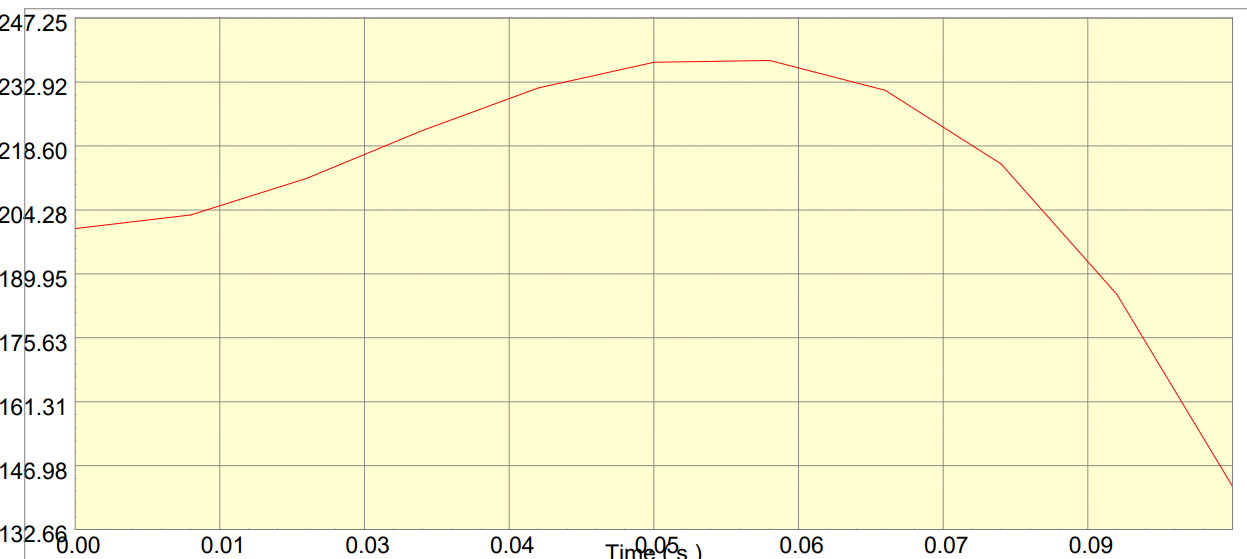
\includegraphics[width=1\linewidth]{inventor/L1_position.png}
    \caption{position over time of L1 end position (x-axis:time(s) , Y-axis: millimeter )}
    \label{fig:enter-label}
\end{figure}

\begin{figure}
    \centering
    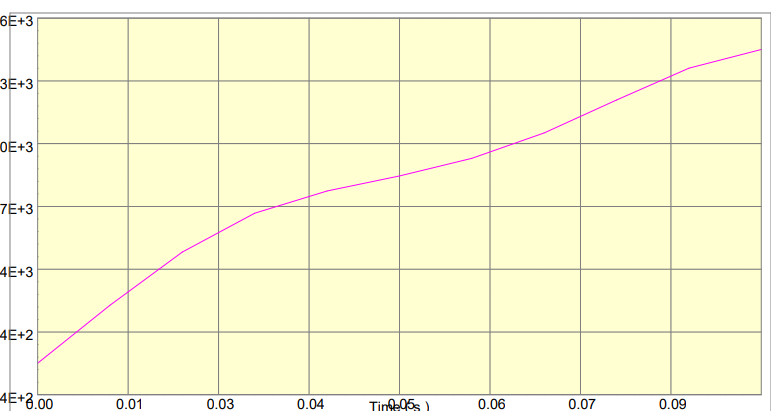
\includegraphics[width=1\linewidth]{inventor/L1_velocity.png}
    \caption{Link 1 velocity over time (x-axis:time(s) , Y-axis: mm/s) }
    \label{fig:enter-label}
\end{figure}
\begin{figure}
    \centering
    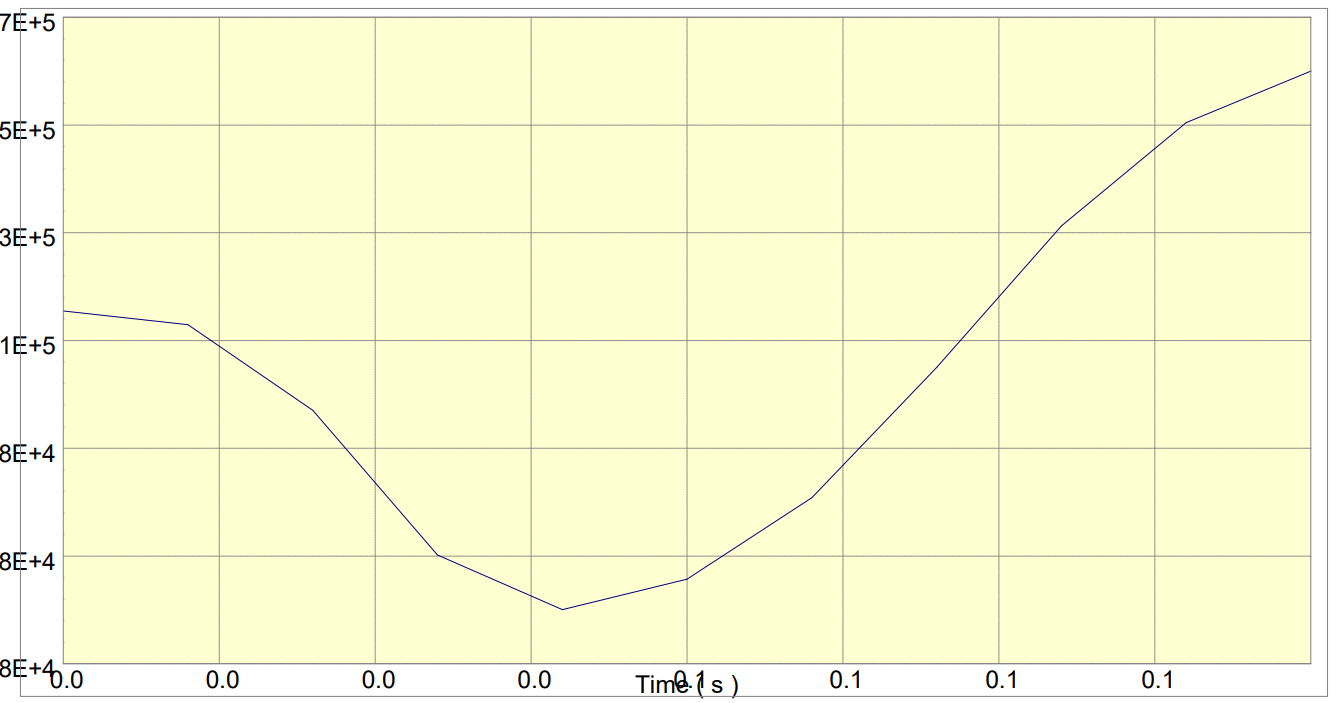
\includegraphics[width=1\linewidth]{inventor/L1_acceleration.png}
    \caption{Link 1 acceleration over time (x-axis:time(s) , Y-axis: $\mathrm{mm/s^2}$) }
    \label{fig:enter-label}
\end{figure}
In the above displayed figure, we present the simulation result  of position, velocity and acceleration of the first link . As we can see the max distance the link L1 travels to is 245 mm from the point of origin which is according to the design parameter of the desired arm implementation. With the configuration, provided the necessary torque at the joint, we plotted velocity and acceleration of link L1 as shown in figure 2 and figure 3 and we can see that the max velocity is 3e10 mm/s and acceleration of  5e5 $\mathrm{mm/s^2}$.  
  
\begin{figure}
    \centering
    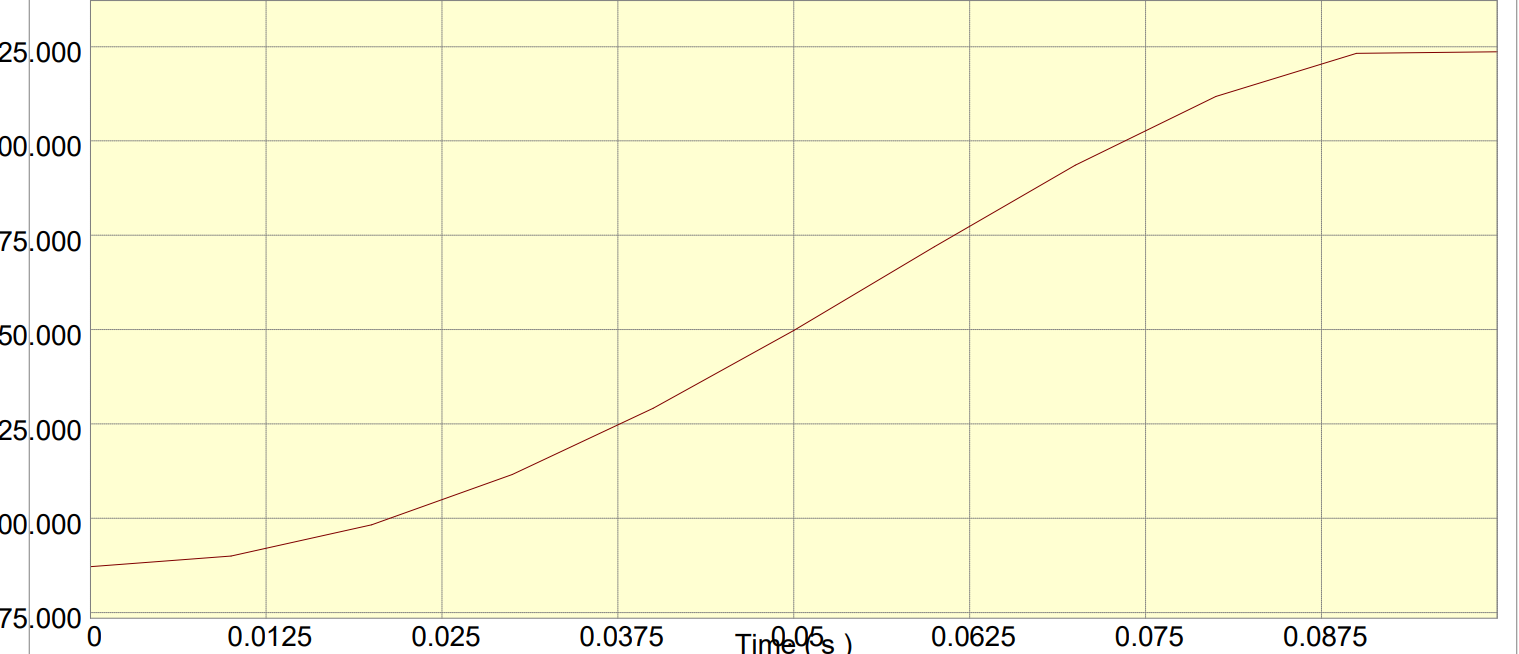
\includegraphics[width=1\linewidth]{inventor/L2_position.png}
    \caption{position over time of L2 end point (x-axis:time(s) , Y-axis: millimeter)}
    \label{fig:enter-label}
\end{figure}

\begin{figure}
    \centering
    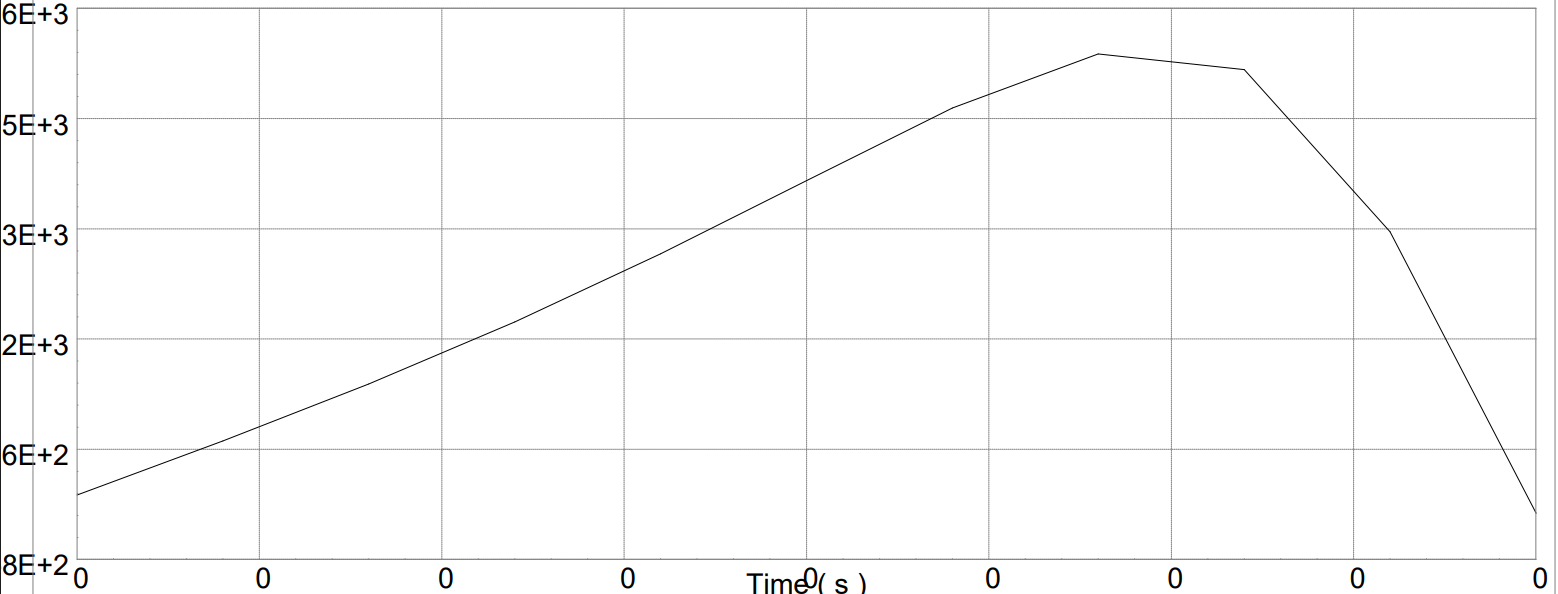
\includegraphics[width=1\linewidth]{inventor/L2_velocity.png}
    \caption{Link 2 velocity over time(x-axis:time(s) , Y-axis: $\mathrm{mm/s}$)}
    \label{fig:enter-label}
\end{figure}
\begin{figure}
    \centering
    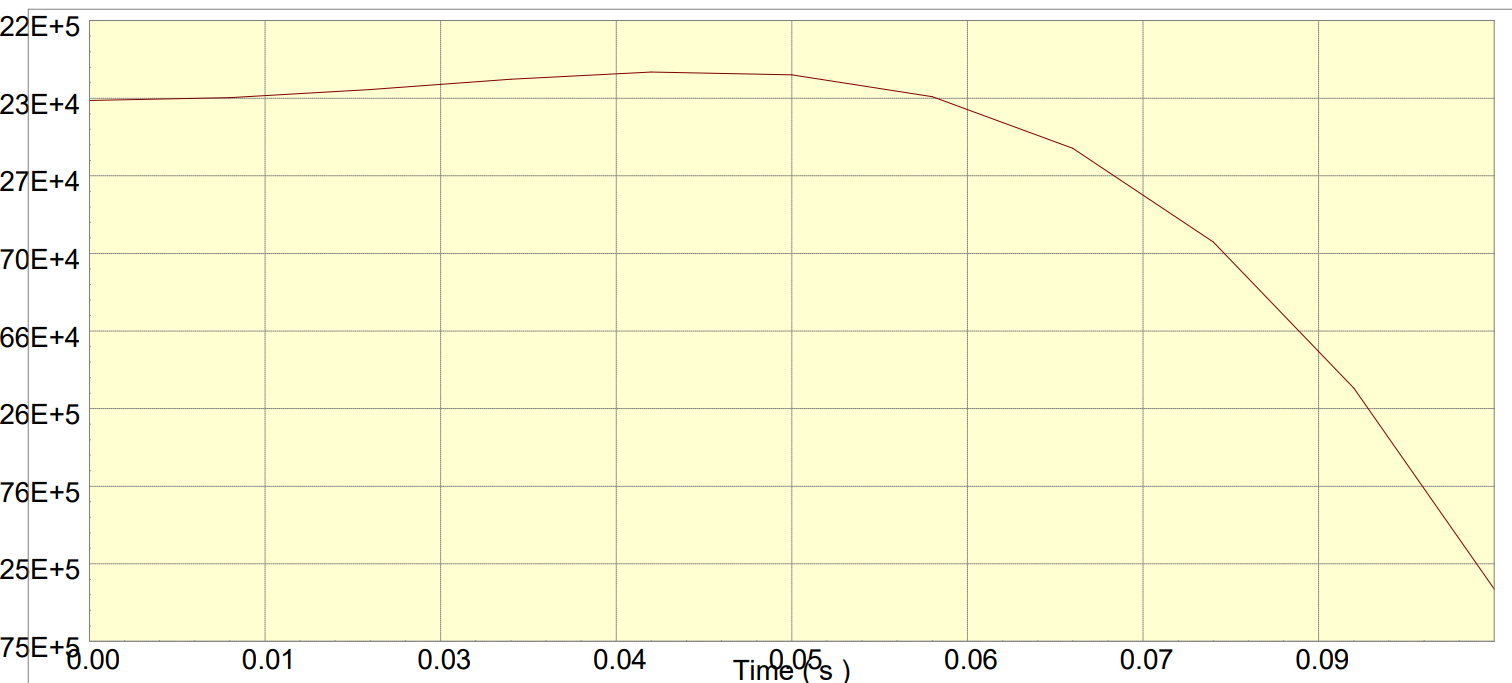
\includegraphics[width=1\linewidth]{inventor/L2_acceleration.png}
    \caption{Link 2 acceleration  over time(x-axis:time(s) , Y-axis: $\mathrm{mm/s^2}$)}
    \label{fig:enter-label}
\end{figure}
simulating the 2nd link L2 gives us the above figures of position and velocity and acceleration. As we can see the position goes to maximum from joint J1 of  25 mm  with max velocity and acceleration of  5e10 $\mathrm{mm/s}$ and 23e4 $\mathrm{mm/s^2}$ respectability.


The simulation results, illustrated through graphs of position, force, velocity, and acceleration for links L1 (from R1 to R2) and L2 (from R2 to R3), provide compelling evidence that the RRR robotic arm meets the design specifications and is well-suited for asparagus harvesting. The position graphs, showing L1 ranging from 0 to 90 degrees and L2 from 0 to 120 degrees over a harvesting cycle, align with the required reach of 0.45 m (0.25 m for L1 and 0.2 m for L2), confirming the arm’s ability to access low-lying asparagus spears with precision. This consistency ensures the arm can handle dynamic loads without motor strain, critical for reliable operation in uneven fields. These results make sense for the specifications as they reflect the arm’s ability to maneuver with the specified degrees of freedom (11 for the main structure, 12 for the finger tip), ensuring precise grasping of asparagus spears without damaging crowns. The data also supports field performance under varying conditions (e.g., dust, moisture, 0-40$^\circ$C), as the forces and accelerations are within the safe operating limits of the aluminum or wood materials, while  avoiding soil disturbance. 
